\section{ベイズ線形回帰 (Bayesian linear regression)}
conjugate prior


\begin{equation}
p(\mathbf{w})=\mathcal{N}(\mathbf{w}|\boldsymbol{\mu}_0, \mathbf{\Sigma}_0)
\end{equation}


posterior


\begin{equation}
p(\mathbf{w}|\mathbf{Y}, \mathbf{X})=\mathcal{N}(\mathbf{w}|\hat{\boldsymbol{\mu}}, \hat{\mathbf{\Sigma}})
\end{equation}


ただし,


\begin{align}
\hat{\mathbf{\Sigma}}^{-1}&= \mathbf{\Sigma}_0^{-1}+ \beta \Phi^\top\Phi\\
\hat{\boldsymbol{\mu}}&=\Sigma_N (\mathbf{\Sigma}_0^{-1}\boldsymbol{\mu}_0+\beta \Phi^\top \mathbf{y})
\end{align}


である.また,$\Phi=\phi.(\mathbf{x})$であり,$\phi(x)=[1, x, x^2, x^3]$, $\boldsymbol{\mu}_0=\mathbf{0}, \mathbf{\Sigma}_0= \alpha^{-1} \mathbf{I}$とする.

テストデータを$\mathbf{x}^*$とした際,予測分布は


\begin{equation}
p(y^*|\mathbf{x}^*, \mathbf{Y}, \mathbf{X})=\mathcal{N}(y^*|\boldsymbol{\mu}^*, \mathbf{\Sigma}^*)
\end{equation}


となる.ただし,


\begin{align}
\boldsymbol{\mu}^*&=\hat{\boldsymbol{\mu}}^\top \phi(\mathbf{x}^*)\\
\mathbf{\Sigma}^* &= \frac{1}{\beta} +  \phi(\mathbf{x}^*)^\top\hat{\mathbf{\Sigma}}\phi(\mathbf{x}^*)\\
\end{align}
\lstinputlisting[language=julia]{./text/bayesian-brain/bayesian-linear-regression/001.jl}
\lstinputlisting[language=julia]{./text/bayesian-brain/bayesian-linear-regression/002.jl}
\lstinputlisting[language=julia]{./text/bayesian-brain/bayesian-linear-regression/003.jl}
\lstinputlisting[language=julia]{./text/bayesian-brain/bayesian-linear-regression/004.jl}
\lstinputlisting[language=julia]{./text/bayesian-brain/bayesian-linear-regression/005.jl}
\begin{figure}[ht]
	\centering
	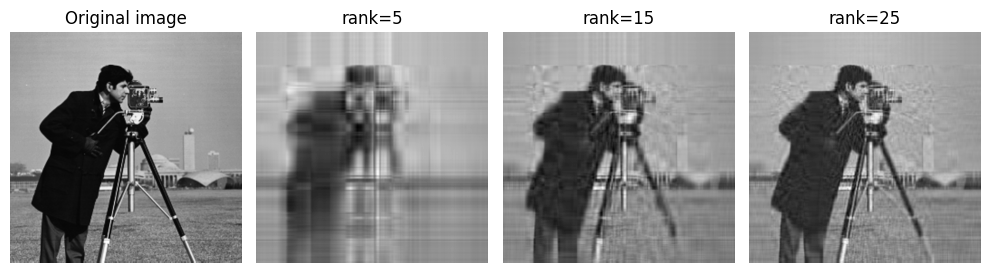
\includegraphics[scale=0.8, max width=\linewidth]{./fig/solve-credit-assignment-problem/linear-network-learning-dynamics/cell005.png}
	\caption{cell005.png}
	\label{cell005.png}
\end{figure}
